\documentclass[11pt, a4paper]{article}

\usepackage{amsmath, amssymb, titling}
\usepackage[margin=2.5cm]{geometry}
\usepackage[colorlinks=true, linkcolor=black, urlcolor=black, citecolor=black]{hyperref}
\usepackage{graphicx}
\usepackage{float}
\usepackage{fancyhdr, lastpage}
\usepackage{xcolor}

\renewcommand\maketitlehooka{\null\mbox{}\vfill}
\renewcommand\maketitlehookd{\vfill\null}

\title{Satellite Orbit Control \\ HW6}
\author{Almog Dobrescu\\\\ID 214254252}

\pagestyle{fancy}
\cfoot{Page \thepage\ of \pageref{LastPage}}

\begin{document}

\maketitle

\thispagestyle{empty}
\newpage
\setcounter{page}{1}

\tableofcontents
\vfil
\listoffigures
\newpage

\section{Given}
\begin{equation*}
    \begin{matrix}
        T_1=100\left[min\right] = 6\cdot10^3\left[sec\right] && T_2 = T_1 = 6\cdot10^3\left[sec\right] \\
        e_1 = 0 && e_2 = 0 \\
        a_1 = \sqrt[3]{\frac{\mu T_1^2}{4\pi^2}} = 7.1366\cdot10^3\left[km\right] && a_2 = a_1 = 7.1366\cdot10^3\left[km\right]
    \end{matrix}\\
\end{equation*}
\begin{equation*}
    \alpha=\Delta i = 0.01^\circ
\end{equation*}
In CW frame with origin at Satellite \#1 and at $t=0$:
\begin{equation*}
    \begin{matrix}
    \begin{pmatrix}
        x_2(0)=0 \\ y_2(0)=-1 \\ z_2(0)=1
    \end{pmatrix}\left[\mathrm{km}\right] &&
    \begin{pmatrix}
        \dot{x}_2(0)=0 \\ \dot{y}_2(0) =0 \\ \dot{z}_2(0)=-0.74267\cdot n
    \end{pmatrix}\displaystyle\left[\frac{\mathrm{km}}{\mathrm{sec}}\right]
    \end{matrix}
\end{equation*}

\subsection{Desired}
\begin{equation*}
    \begin{matrix}
    \begin{pmatrix}
        x_2(t_f)=0 \\ y_2(t_f)=0 \\ z_2(t_f)=0
    \end{pmatrix} &&
    \begin{pmatrix}
        \dot{x}_2(t_f)=0 \\ \dot{y}_2(t_f)=0 \\ \dot{z}_2(t_f)=0
    \end{pmatrix}
    \end{matrix}
\end{equation*}

\subsection{Limitations}
\begin{equation*}
    \begin{matrix}
        a_\text{max} = 4\cdot10^{-5}\left[\frac{\mathrm{km}}{\mathrm{sec}^2}\right] && t_f=2000\left[sec\right]
    \end{matrix}
\end{equation*}

\section{The CW equations}
\begin{equation}
    \left\{\begin{array}{l}
        \ddot{x}-2n\dot{y}-3n^2x=f_x\\
        \ddot{y}+2n\dot{x}=f_y\\
        \ddot{z}+n^2z=f_z
    \end{array}\right.
\end{equation}

\subsection{x-y}
\begin{equation}
    \vec{x}=\begin{pmatrix}
        x\\\dot{x}\\y\\\dot{y}
    \end{pmatrix}
\end{equation}
\begin{equation}
    \dot{\vec{x}}=F\vec{x}+G\vec{f}
\end{equation}
Where:
\begin{equation}
    \begin{matrix}
        F=\begin{pmatrix}
            0 & 1 & 0 & 0 \\
            3n^2 & 0 & 0 & 2n \\
            0 & 0 & 0 & 1 \\
            0 & -2n & 0 & 0
        \end{pmatrix} && G=\begin{pmatrix}
            0 & 0\\
            1 & 0\\
            0 & 0\\
            0 & 1
        \end{pmatrix} && f=\begin{pmatrix}
            f_x\\f_y
        \end{pmatrix}
    \end{matrix}
\end{equation}

\subsection{z}
\begin{equation}
    \vec{x}=\begin{pmatrix}
        z\\\dot{z}
    \end{pmatrix}
\end{equation}
\begin{equation}
    \dot{\vec{x}}=F\vec{x}+Gf
\end{equation}
Where:
\begin{equation}
    \begin{matrix}
        F=\begin{pmatrix}
            0 & 1 \\
            -n^2 & 0
        \end{pmatrix} && G=\begin{pmatrix}
            0 \\
            1
        \end{pmatrix} && f=\begin{pmatrix}
            f_z
        \end{pmatrix}
    \end{matrix}
\end{equation}

\subsection{x-y-z}
The equations of motion in state space form are therefor:
\begin{equation}
    \vec{x} = \begin{pmatrix}
        x & \dot{x} & y & \dot{y} & z & \dot{z}
    \end{pmatrix}^T
\end{equation}
\begin{equation}
    \dot{\vec{x}}=F\vec{x}+G\vec{f}
\end{equation}
Where:
\begin{equation}
    \begin{matrix}
        F=\begin{pmatrix}
            0 & 1 & 0 & 0 & 0 & 0 \\
            3n^2 & 0 & 0 & 2n & 0 & 0 \\
            0 & 0 & 0 & 1 & 0 & 0 \\
            0 & -2n & 0 & 0 & 0 & 0 \\
            0 & 0 & 0 & 0 & 0 & 1 \\
            0 & 0 & 0 & 0 & -n^2 & 0 
        \end{pmatrix} && G=\begin{pmatrix}
            0 & 0 & 0\\
            1 & 0 & 0\\
            0 & 0 & 0\\
            0 & 1 & 0\\
            0 & 0 & 0\\
            0 & 0 & 1
        \end{pmatrix} && f=\begin{pmatrix}
            f_x\\f_y\\f_z
        \end{pmatrix}
    \end{matrix}
\end{equation}

\section{LQR}
The linear system:
\begin{equation}
    \begin{matrix}
        \dot{\vec{x}}=F\vec{x}+G\vec{u} && \vec{x}_{\left(t_0\right)}=\vec{x}_0
    \end{matrix}
\end{equation}
It is needed to find a controler to bring the system to the end position while minimaizing the cost cratiria:
\begin{equation}
    J=\frac{1}{2}\vec{x}_f^TP_f\vec{x}_f+\frac{1}{2}\int_0^{t_f}\left(\vec{x}^TQ\vec{x}+\vec{u}^TR\vec{u}\right)dt
\end{equation}
$P_f,Q,R$ are PD matrices that the users chose w.r.t. the requierments and limitations.\\
The Hamiltonian:
\begin{equation}
    H=\vec{x}^TQ\vec{x}+\vec{u}^TR\vec{u}+\vec{\lambda}^T\left(F\vec{x}+G\vec{u}\right)
\end{equation}
The optimum condition:
\begin{equation}
    \begin{matrix}
        \displaystyle\frac{\partial H}{\partial \vec{u}}=0 && \rightarrow && \vec{u}=-R^{-1}G^T\vec{\lambda}
    \end{matrix}
\end{equation}
The Euler Lagrange equations:
\begin{equation}
    \begin{matrix}
        \displaystyle\dot{\vec{\lambda}}^T=-\frac{\partial H}{\partial\vec{x}} && \rightarrow && \dot{\vec{\lambda}}=-Q\vec{x}-F^T\vec{\lambda}, && \displaystyle\vec{\lambda}_f^T=\frac{\partial J}{\partial\vec{x}_f}=\vec{x}_f^TP_f
    \end{matrix}
\end{equation}
By combining both equations we get:
\begin{equation}
    \begin{pmatrix}
        \dot{\vec{x}} \\ \dot{\vec{\lambda}}
    \end{pmatrix}=\begin{pmatrix}
        F & -GR^{-1}G^T \\
        -Q & -F^T
    \end{pmatrix}\begin{pmatrix}
        \vec{x} \\ \vec{\lambda}
    \end{pmatrix}
\end{equation}
We can write the system like:
\begin{equation}
    \Phi_{\left(t,t_0\right)}=\begin{pmatrix}
        \Phi_{11\left(t,t_0\right)} & \Phi_{12\left(t,t_0\right)} \\
        \Phi_{21\left(t,t_0\right)} & \Phi_{22\left(t,t_0\right)}
    \end{pmatrix}
\end{equation}
Using the transion matrix, the instantaneous state vector w.r.t the final state:
\begin{equation}
    \begin{matrix}
        \vec{x}_{\left(t\right)}=\Phi_{11\left(t,t_f\right)}\vec{x}_f+\Phi_{12\left(t,t_f\right)}\vec{\lambda}_f \\
        \begin{matrix}
           &&&&&&&& \Downarrow & \left(\vec{\lambda}_f=P_f^T\vec{x}_f\right)
        \end{matrix} \\
        \vec{x}_{\left(t\right)}=\left(\Phi_{11\left(t,t_f\right)}+\Phi_{12\left(t,t_f\right)}P_f^T\right)\vec{x}_f
    \end{matrix}
\end{equation}
Likewise:
\begin{equation}
    \vec{\lambda}_{\left(t\right)}=\left(\Phi_{21\left(t,t_f\right)}+\Phi_{22\left(t,t_f\right)}P_f^T\right)\vec{x}_f
\end{equation}
By combining the equations, we can get a linear conection between $\vec{x}\mathrm{\ and\ }\vec{\lambda}$:
\begin{equation}
    \vec{\lambda}_{\left(t\right)}=\left(\Phi_{21\left(t,t_f\right)}+\Phi_{22\left(t,t_f\right)}P_f^T\right)\left(\Phi_{11\left(t,t_f\right)}+\Phi_{12\left(t,t_f\right)}P_f^T\right)^{-1}\vec{x}_{\left(t\right)}\equiv P_{\left(t\right)}\vec{x}_{\left(t\right)}
\end{equation}
The porpotional controler will be writen as:
\begin{equation}
    \begin{matrix}
        \vec{u}_{\left(t\right)}=-K_{\left(t\right)}\vec{x}_{\left(t\right)}, && K_{\left(t\right)}=R^{-1}G^TP_{\left(t\right)}
    \end{matrix}
\end{equation}
In order to find the matrix \emph{P} we will substitut $\vec{\lambda}=P\vec{x}$ inside the Euler Lagrange equations:
\begin{equation}
    \begin{matrix}
        \dot{P}\vec{x}+P\dot{\vec{x}}=-Q\vec{x}-F^TP\vec{x} \\
        \Downarrow \\
        \left(\dot{P}+PF+F^TP-PGR^{-1}G^TP+Q\right)\vec{x}=0
    \end{matrix}
\end{equation}
The equation is right for every \emph{x} so:
\begin{equation}
    \begin{matrix}
        \dot{P}+PF+F^TP-PGR^{-1}G^TP+Q=0, && P_{\left(t_f\right)}=P_f
    \end{matrix}
\end{equation}
This is the 'matrix Rikati equation'
\newpage

\section{The Gains Matrix}
Setting $Q,R$ to be:
\begin{equation}
    \begin{matrix}
        Q=\begin{pmatrix}
            \displaystyle\frac{1}{x_{\mathrm{miss}}^2} & 0 & 0 & 0 & 0 & 0 \\
            0 & \displaystyle\frac{1}{v_{\mathrm{miss}}^2} & 0 & 0 & 0 & 0 \\
            0 & 0 & \displaystyle\frac{1}{x_{\mathrm{miss}}^2} & 0 & 0 & 0 \\
            0 & 0 & 0 & \displaystyle\frac{1}{v_{\mathrm{miss}}^2} & 0 & 0 \\
            0 & 0 & 0 & 0 & \displaystyle\frac{1}{x_{\mathrm{miss}}^2} & 0 \\
            0 & 0 & 0 & 0 & 0 & \displaystyle\frac{1}{v_{\mathrm{miss}}^2}
        \end{pmatrix} && \displaystyle R=\frac{1}{f_{max}^2}
    \end{matrix}
\end{equation}
By using the function \emph{lqr} in Matlab, we get:
\begin{equation}
    K = \begin{pmatrix}
        0.0400&4.0100&-0.0000&0.0000&-0.0000&-0.0000\\
        0.0000&0.0000&0.0400&4.0100&0.0000&0.0000\\
        0.0000&0.0000&-0.0000&-0.0000&0.0400&4.0100
    \end{pmatrix}
\end{equation}

\section{The Results}
\begin{figure}[H]
    \centering
    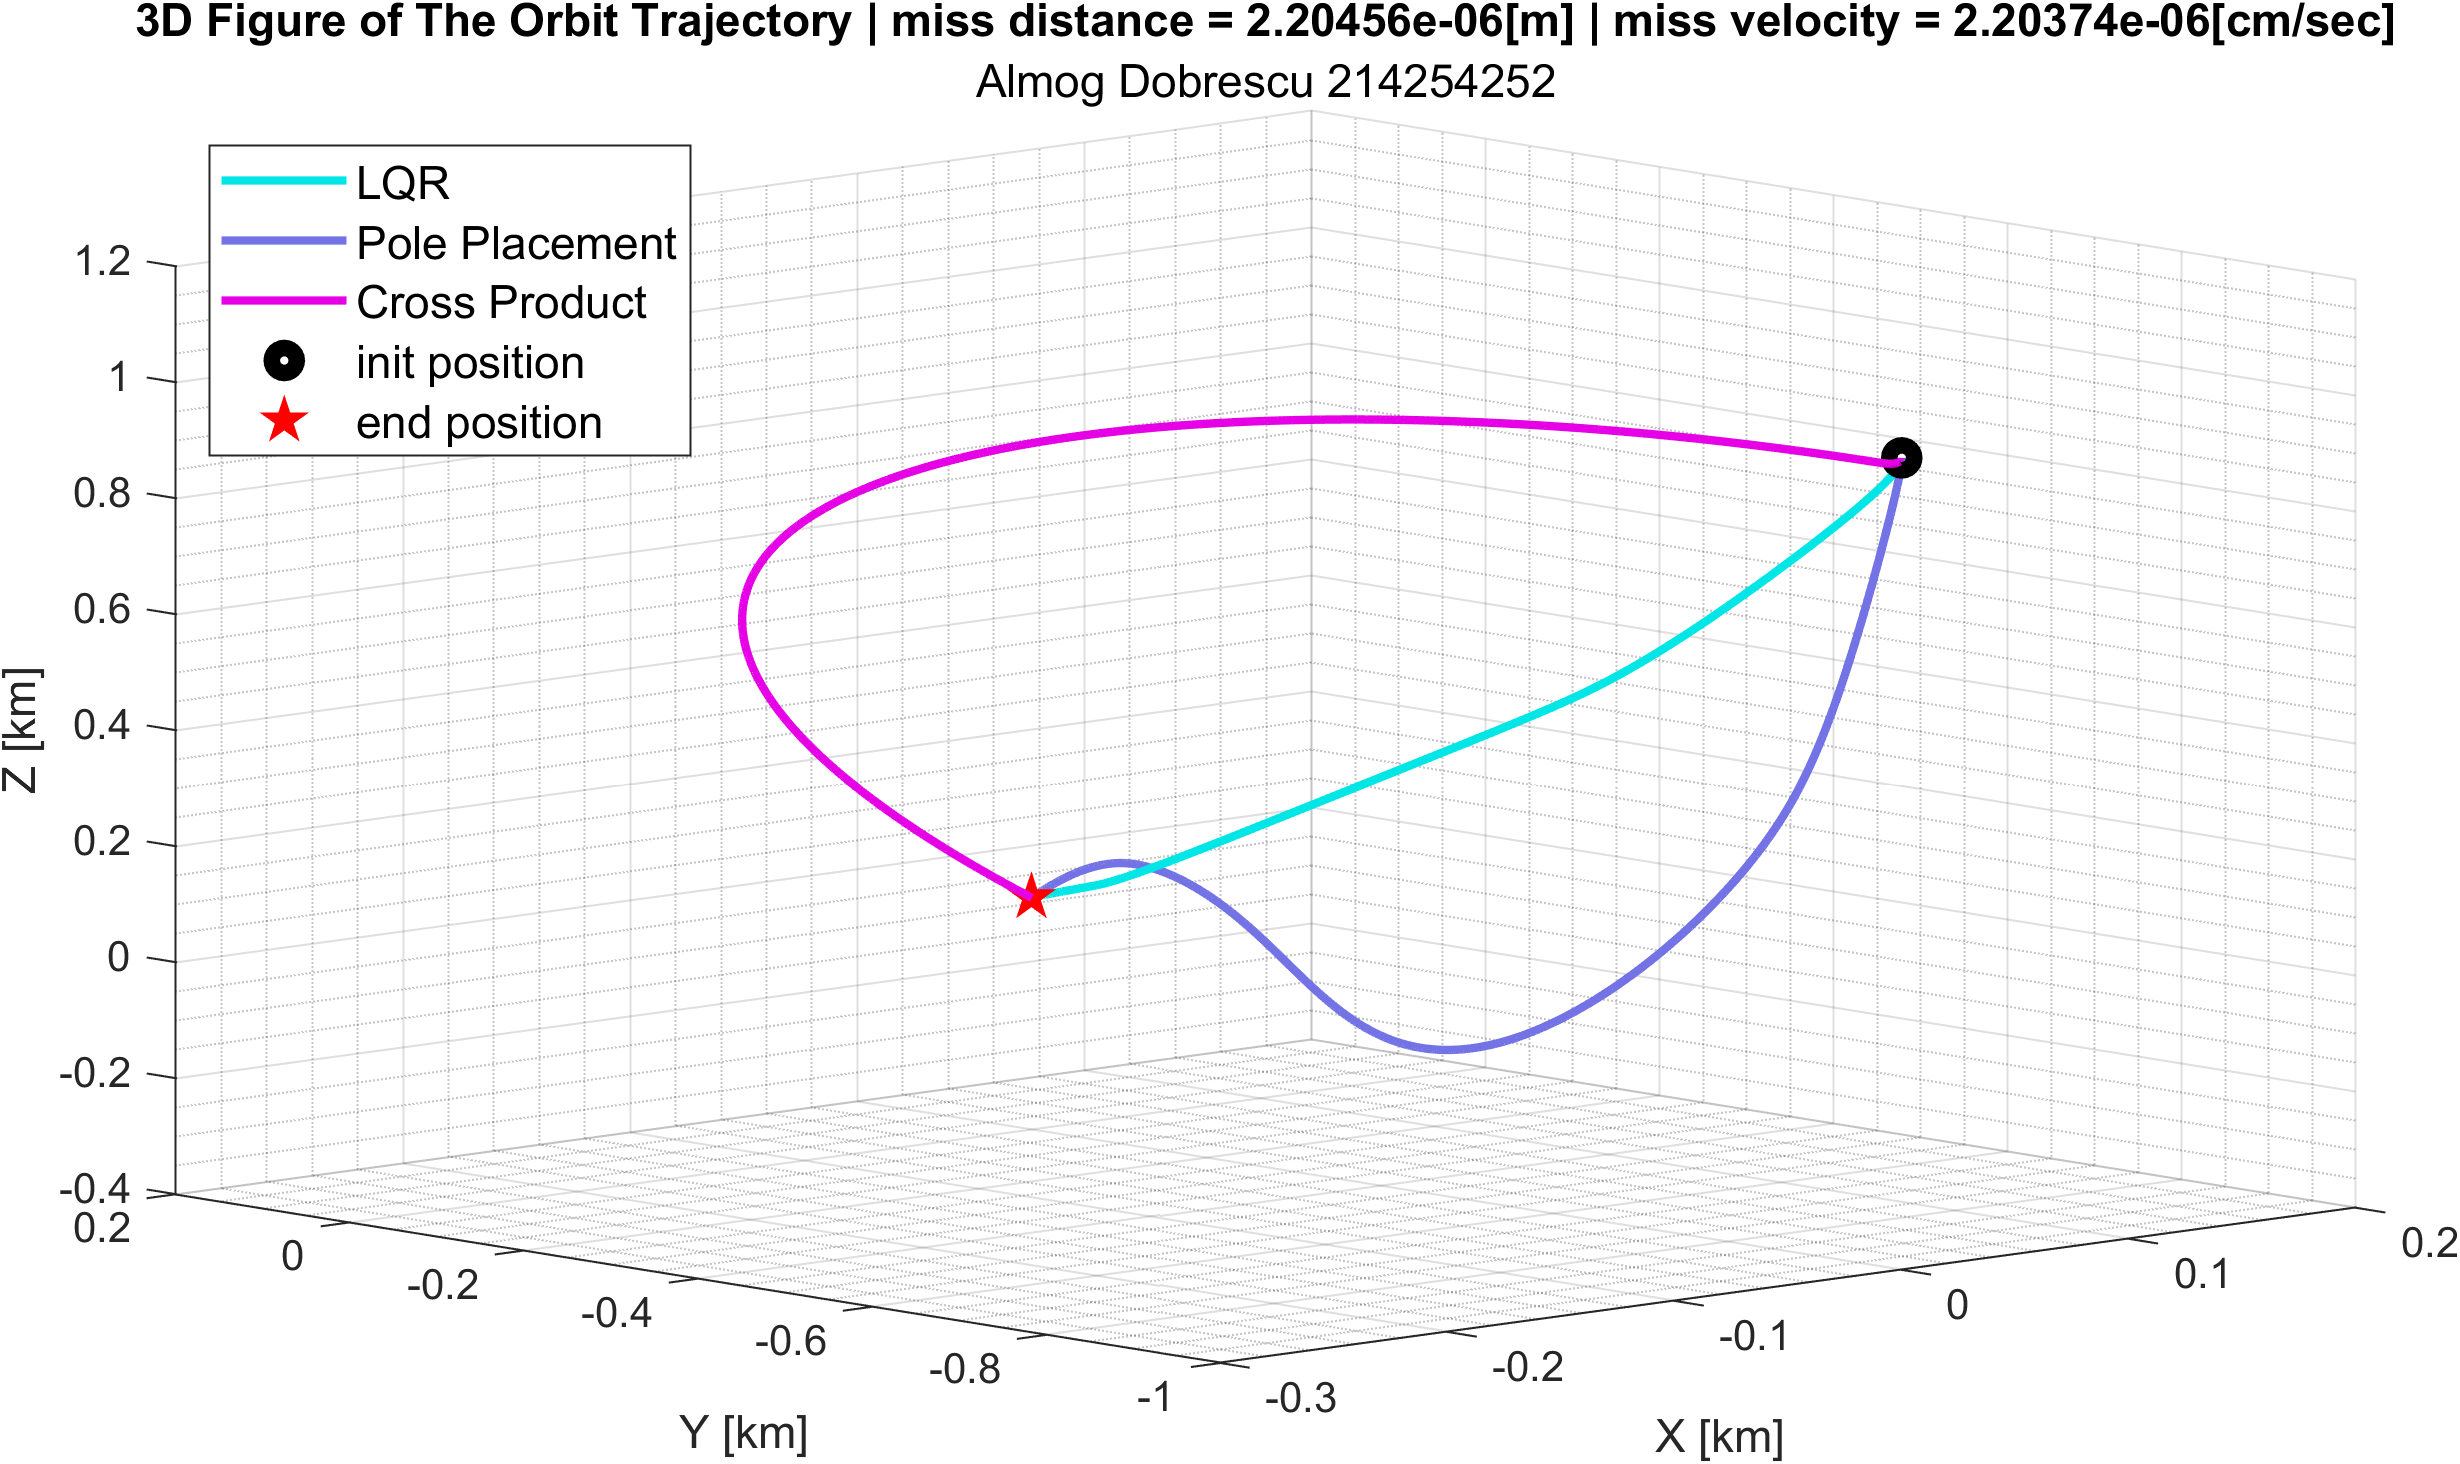
\includegraphics[width=1\textwidth]{images/graph1.png}
    \caption{3D figure of the orbit trajectory}
    \label{fig:3D-plot}
\end{figure}
\begin{figure}[H]
    \centering
    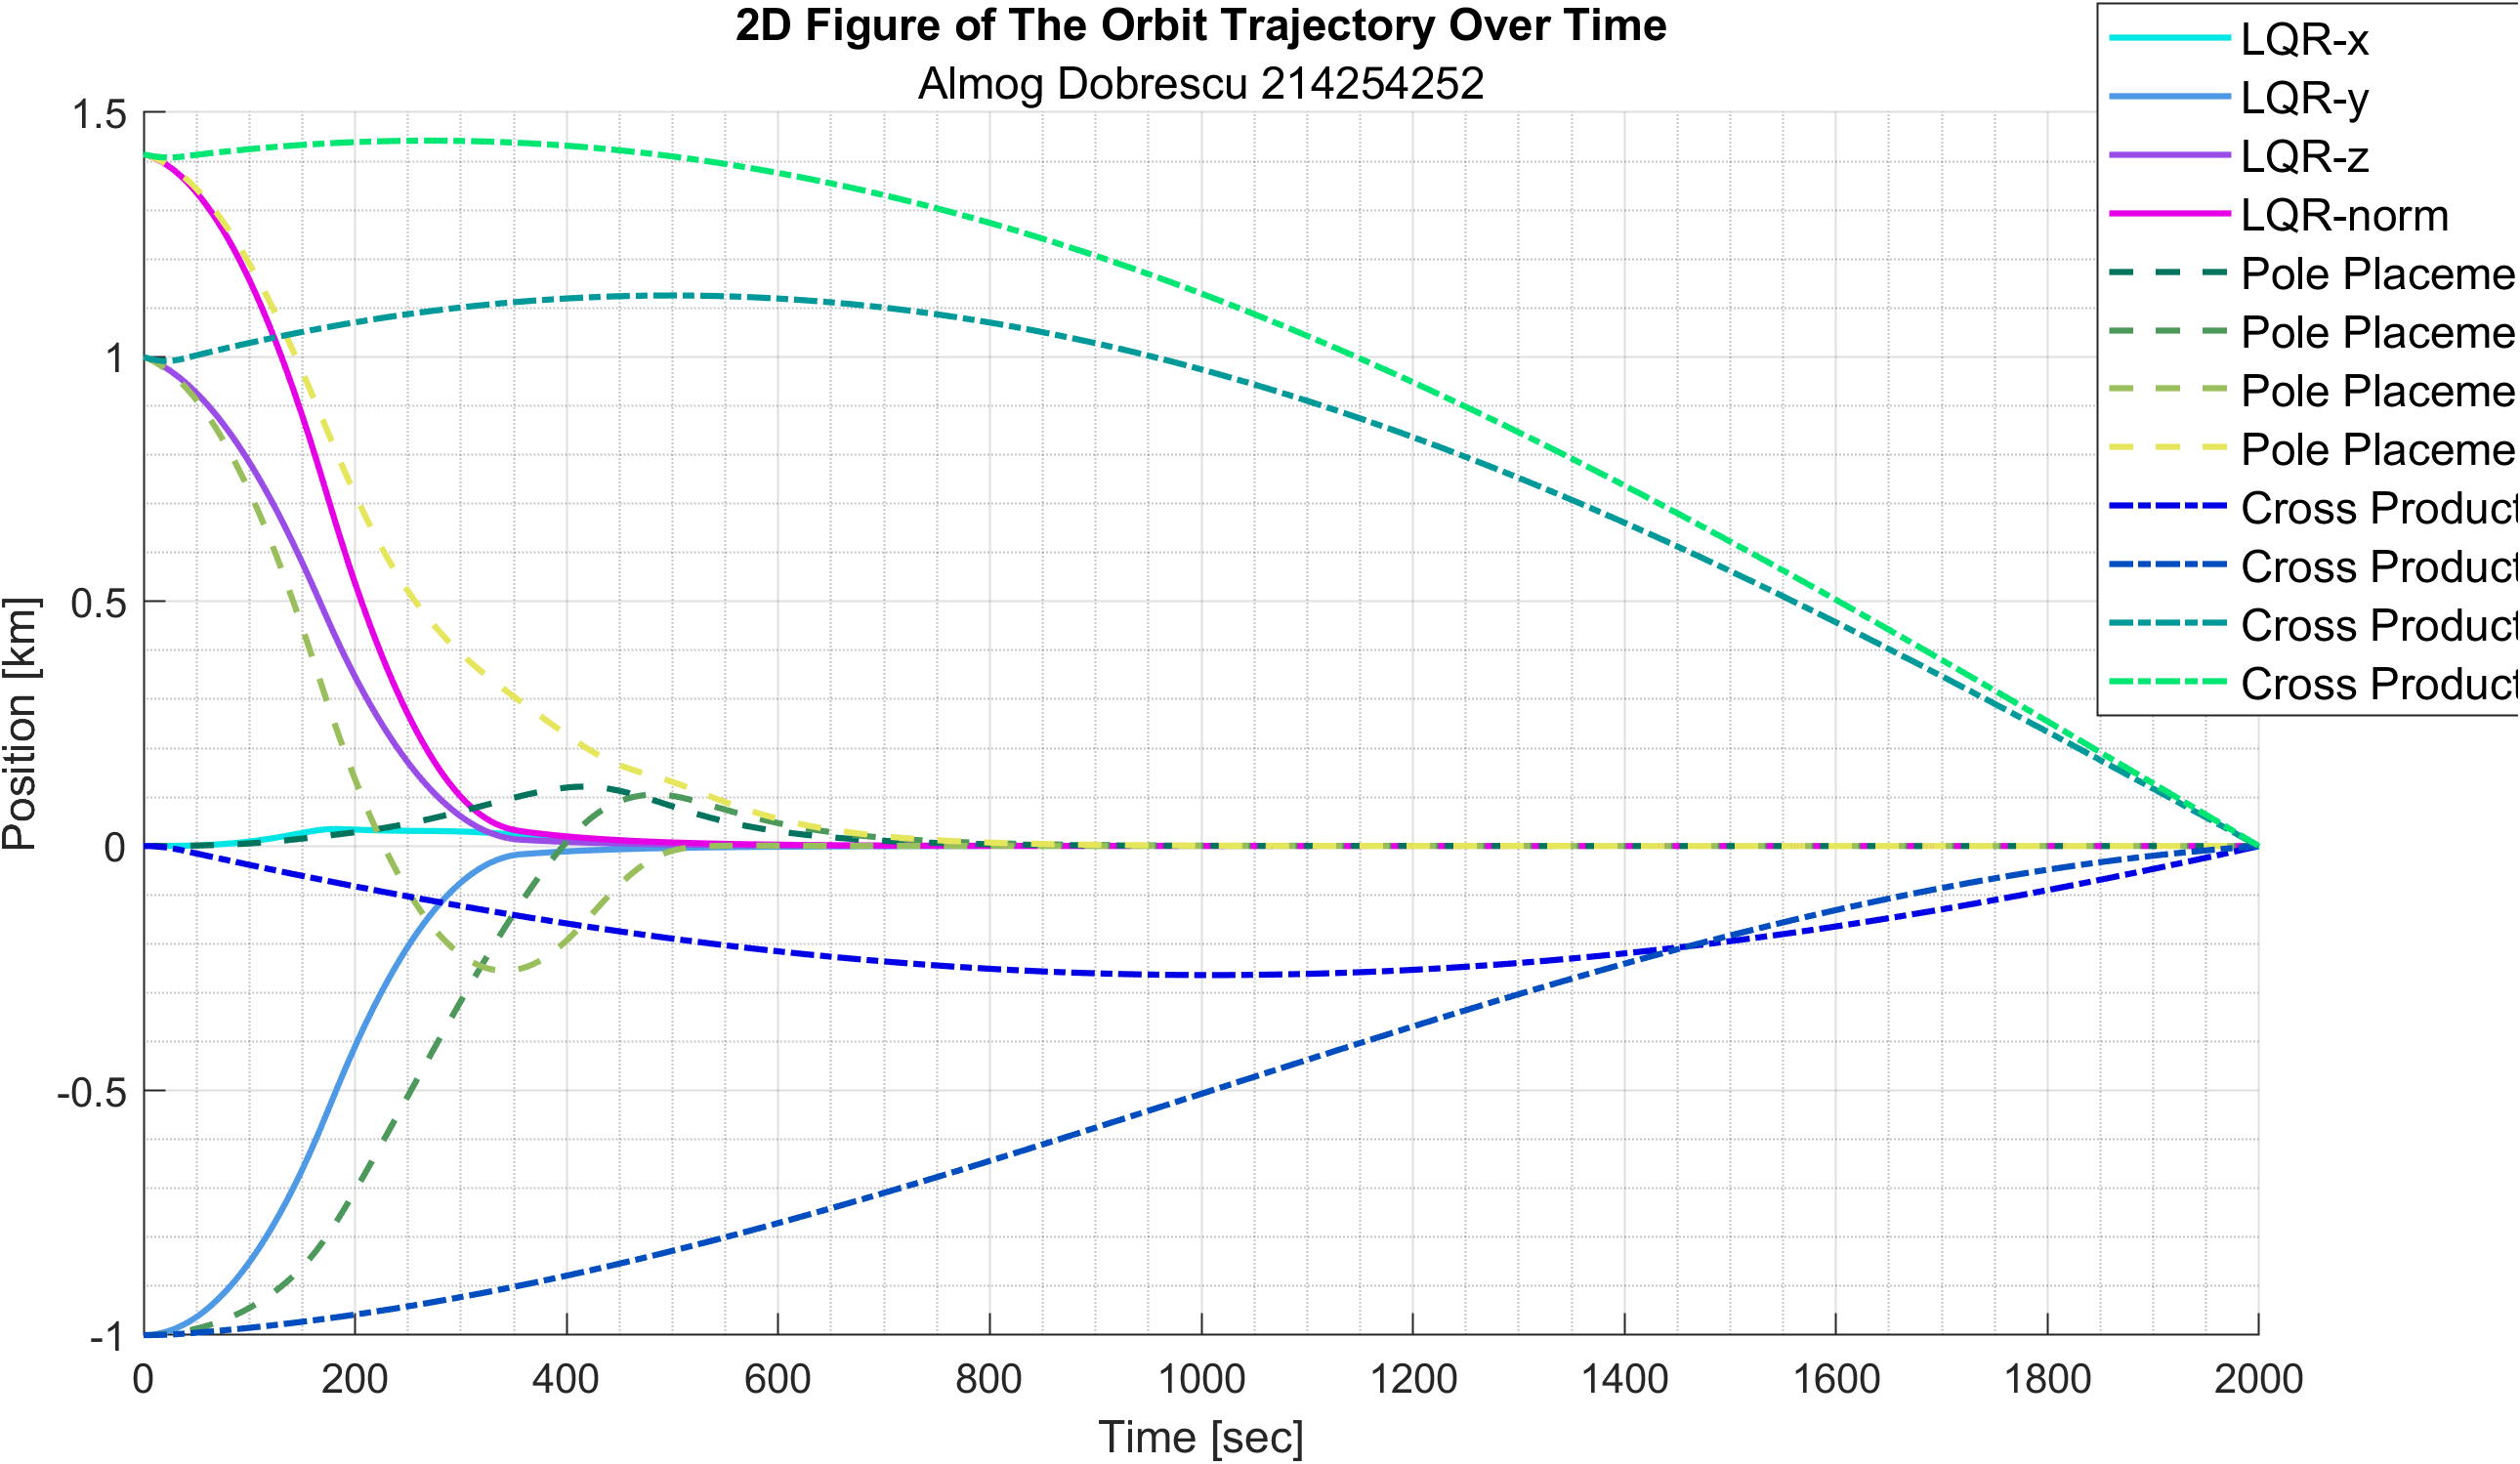
\includegraphics[width=1\textwidth]{images/graph2.png}
    \caption{2D figure of the orbit target trajectory over time}
    \label{fig:2D-plot_over_time}
\end{figure}
\begin{figure}[H]
    \centering
    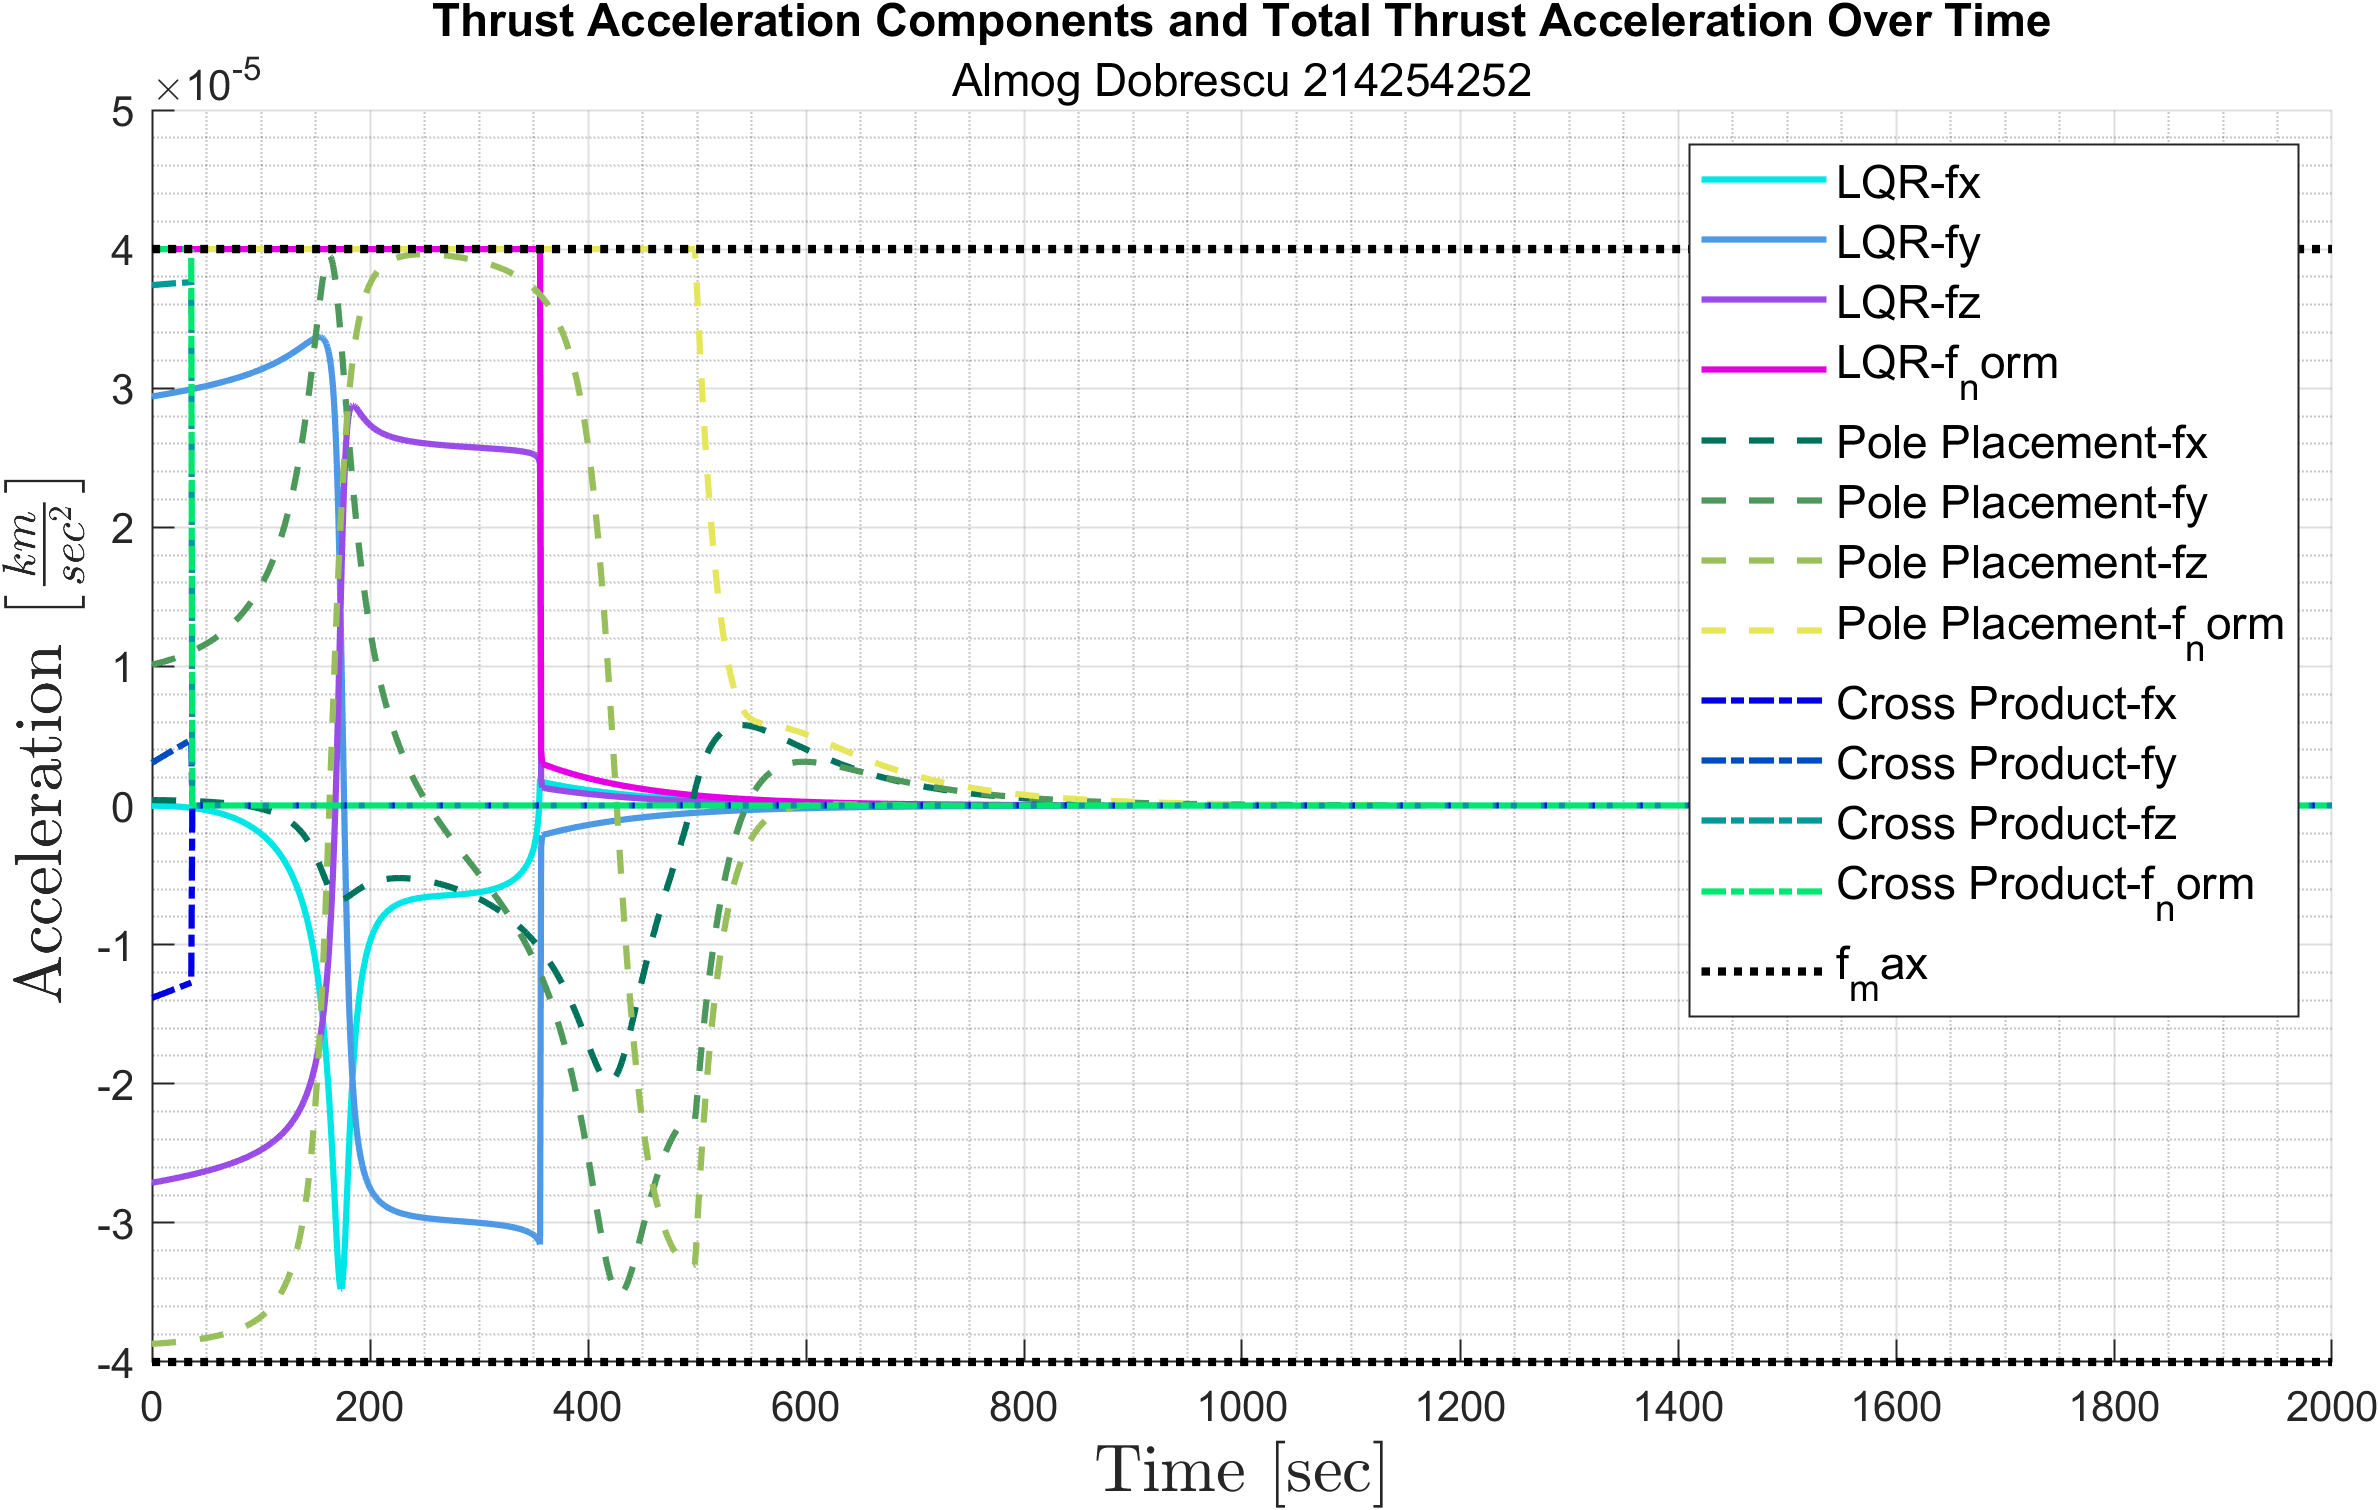
\includegraphics[width=1\textwidth]{images/graph3.png}
    \caption{Thrust acceleration components and total thrust acceleration over time}
    \label{fig:accel_over_time}
\end{figure}
\begin{figure}[H]
    \centering
    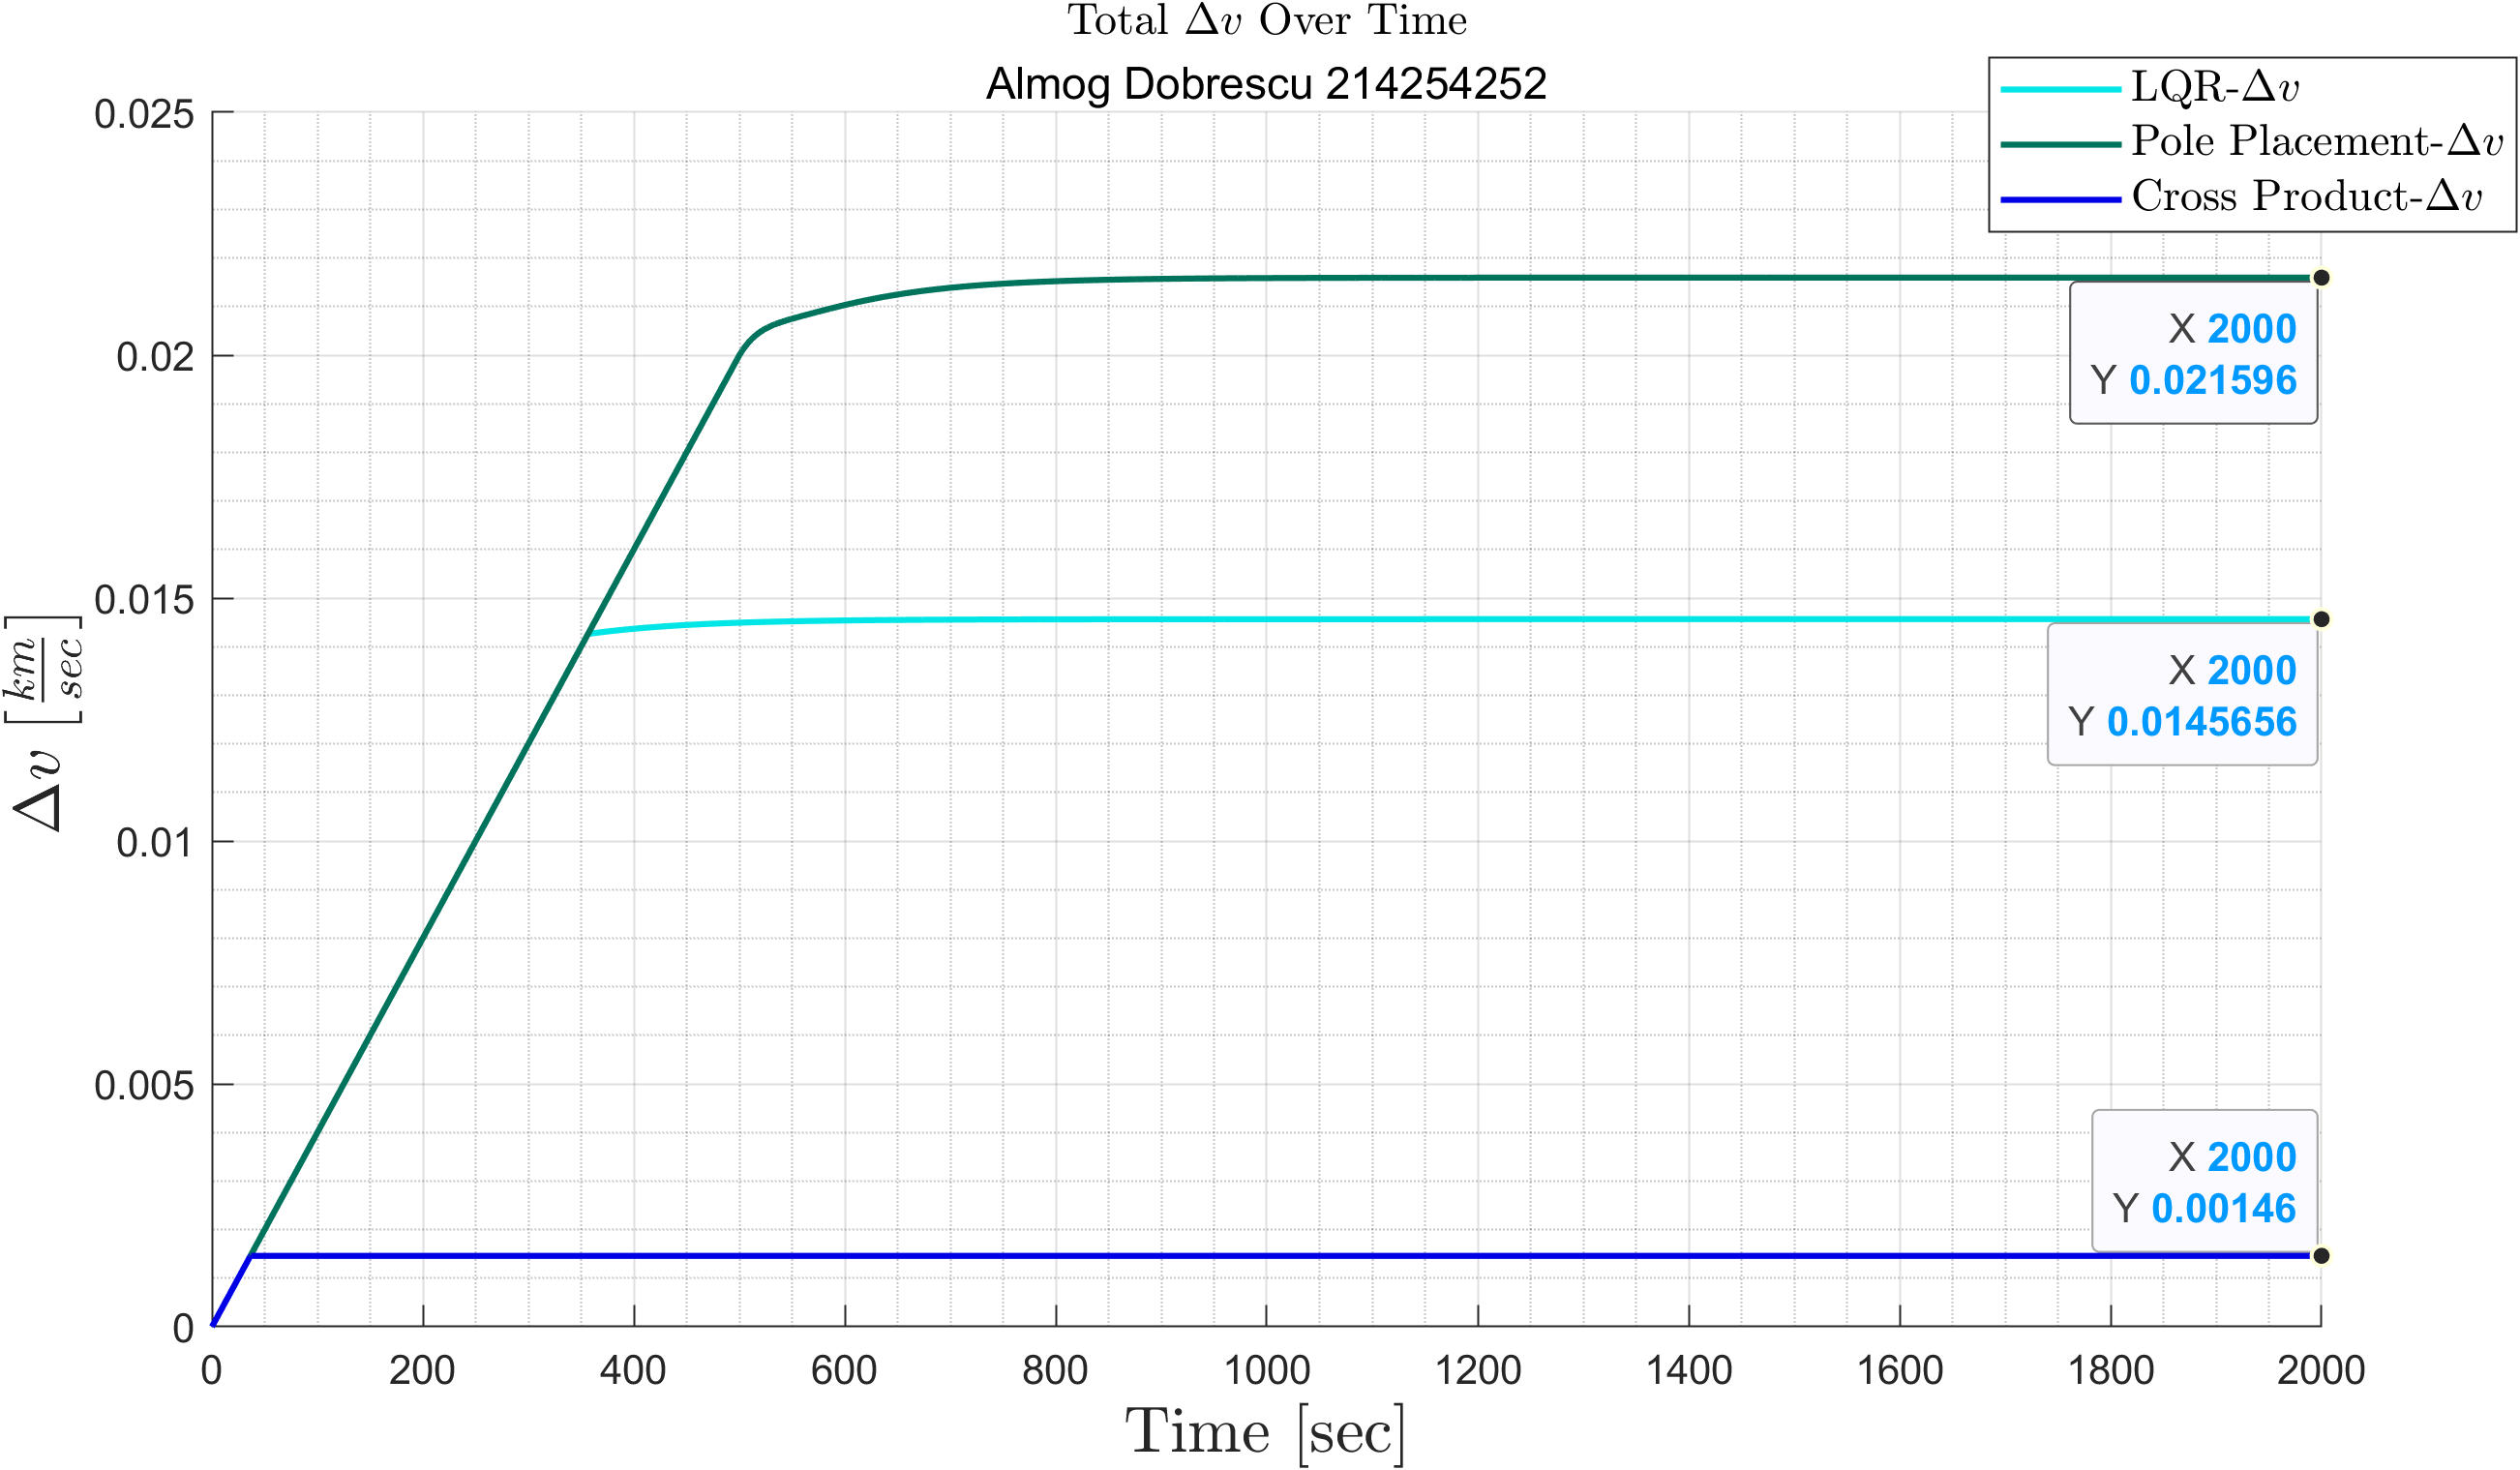
\includegraphics[width=1\textwidth]{images/graph4.png}
    \caption{Total $\Delta v$ over time}
    \label{fig:delta_v_over_time}
\end{figure}
We can see that we indeed acomplished the design criteria:
\begin{itemize}
    \item The thrust doesn't exceed the maximum available thrust.
    \item The miss distance at the final desired time is less than $1[\mathrm{m}]\ \left(2.2047\cdot10^{-6}\left[\mathrm{m}\right]\right)$.
    \item The miss velocity at the final desired time is less than $1\left[\displaystyle\frac{\mathrm{cm}}{\mathrm{sec}}\right]\ \left(2.2037\cdot10^{-6}\left[\displaystyle\frac{\mathrm{cm}}{\mathrm{sec}}\right]\right)$.
\end{itemize}

The total $\Delta v$ is: $0.0146\left[\displaystyle\frac{\mathrm{km}}{\mathrm{sec}}\right]$

\end{document}